\chapter{Einführung}
\label{cha:Einfuehrung}

Der technologische Prozess einer Kältemaschine ermöglicht es einer Wärmequelle Wärme  auf einem niedrigen Temperaturniveau zu entziehen und diese an eine Wärmesenke auf einem höheren Temperaturniveau wieder abzugeben. Um diesen thermodynamischen Prozess zu ermöglichen, muss dem  Kältekreislauf, nach dem 2. Hauptsatz der Thermodynamik, Energie hinzugefügt werden. 

Im Jahre 2009 waren alleine in Deutschland 129 Millionen Kältemaschinen in Gebrauch. 70$\%$ Prozent dieser Kältemaschinen wurden elektrisch angetrieben. Folglich ist die wichtigste Technologie zur Erzeugung von Kälte die Kompressionskälteanlage. Der Energieverbrauch für den Betrieb dieser Anzahl an Kältemaschine beliefen sich 2009 nach Schätzungen von \citeauthor{Preuss2011} auf  ca. 72 Mrd. kWh . Dies entspricht ca. 15 $\%$ des nationalen Stromverbrauchs. Die Aufteilung der Kältemaschinen auf ihre Einsatzbereich ist in Abbildung \ref{fig:Aufteilung nach Einsatzgebiet} dargestellt. \citep{M.Stoeckner2012} \citep{EnergieAgenturNRW2010}

\begin{figure}[htb]
	\centering
		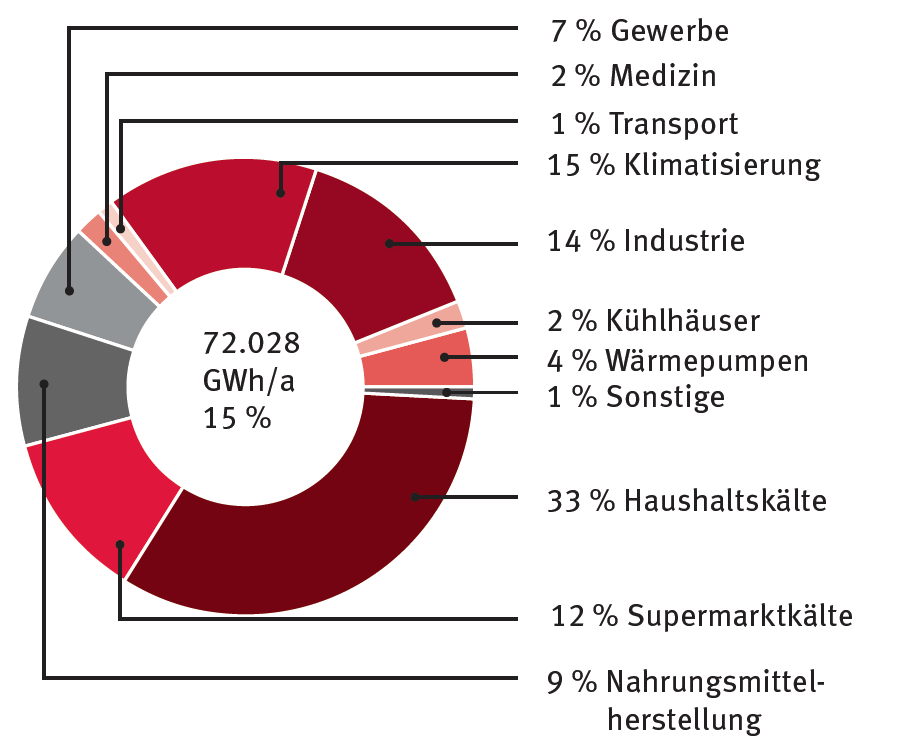
\includegraphics[width=0.570\textwidth]{Pictures/Energieverbrauch_Aufteilung_Karlsruhe.png}
	\caption{Aufteilung der sich in Deutschland in Betrieb befindenden Kältemaschinen je nach Einsatzgebiet und Energieverbrauch im Jahre 2009. \citep{M.Stoeckner2012}}
	\label{fig:Aufteilung nach Einsatzgebiet}
\end{figure}

Der Kälteleistungsbedarf ist nach wie vor ansteigend, womit eine größere Klimabelastung einhergeht. Auf der einen Seite entsteht eine steigende CO$_{2}$ Belastung für die Bereitstellung der Antriebsenergie der Kältemaschinen. Auf der anderen Seite stellt die Belastung der Umwelt durch ungewollte direkte Kältemittelemissionen mit teils hohen CO2-Äquivalenten Emissionen eine Herausforderung dar.

%Das Energiekonzept 2010 der deutschen Bundesregierung setzt die Umweltziele der Zukunft fest. Gegenüber dem Jahr 1990 sollen bis 2020 40$\%$ und bis 2050 $\%80$ der Treibhausgasemissionen eingespart werden. Der Primärenergieverbrauch, bezogen auf das Jahr 2008 ,soll um 20$\%$  bis ins Jahr 2020 und bis 2050 sogar auf 50$\%$ reduziert werden. \citep{BMWi2010}

%\begin{figure}[htb]
%	\centering
%		\includegraphics[width=.960\textwidth]{Pictures/%Energieeinsparpotentiale_Pehnt.png}
%\caption{Energieeinsparpotentiale bis 2030 für die Sektoren Haushalt, Gewerbe 		%und Handel, Verkehr und Industrie.  \citep{Pehnt2011}}
%	\label{fig:Energieeinsparpotentiale}
%	\label{fig:Aufteilung nach Einsatzgebiet}
%\end{figure}

%Um diese Ziele zu erreichen hat \citeauthor{Pehnt2011} einen Maßnahmencluster bestehend aus 42 potentielle Maßnahmen zur Energieeinsparung für Deutschland erstellt. Zunächst sind alle Endverbraucher in 4 Gruppen und die Endenergie in 4 Gruppen unterteilt worden. Jeder Maßnahme wird ein \textit{politischer Handlungsbedarf} bezüglich politischer Instrumente zugeteilt. Dabei wird dem Endenergie-Bereich \textit{Wärme und Kälte} ein \textit{mittleres} bis \textit{großes} Energieeinsparungspotential zugerechnet. 


Im Bezug auf Kältemaschinen werden in der Literatur eine Vielzahl an Möglichkeiten und Potentialabschätzungen zur Senkung des Energieverbrauches und der Umweltbelastung genannt. Von der Verwendung von natürlichem Kältemittel, Wärmerückgewinnung vom Verflüssiger sowie von Downsizing des Kompressors ist die Rede. Laut \textsc{\citeauthor{EnergieAgenturNRW2010}} entfallen bei der elektrischen Leistungsaufnahme einer Kälteanlage im Kühlbetrieb durchschnittlich:

\begin{itemize}
	\item ca.88 $\%$ auf den Kompressor,
	\item ca. 7 $\%$ auf den Verflüssiger,
	\item ca. 5 $\%$ auf den Verdampfer.
\end{itemize}

Die Energieverbrauch des Verflüssigers bzw. Verdampfers wird durch deren eingebauten Ventilator bestimmt. 
Folglich ist der Kompressor der größte Energieverbaucher in einer Kälteanlage. Um eine effiziente Kälteanlage zu betreiben, sollte die zu verrichtende Arbeit vom Kompressor so niedrig wie möglich gehalten werden.

In dieser Arbeit sollen verschiedene Abtaumethoden für einen vereisten Luftkühler näher untersucht werden, da diese im direkten Zusammenhang mit der Leistungsaufnahme des Kompressors stehen. Vereiste Luftkühler führen zu einem Leistungsabfall sowie zu einem erhöhten Stromverbrauch durch den Kompressor. Dadurch muss der Luftkühler zu bestimmten Zeiten abgetaut werden, um das Eis von dem Wärmeübertrager zu entfernen und die ursprüngliche Kälteleistung wieder zur Verfügung stellen zu können. 



